\documentclass[11pt]{article}
\usepackage{colacl}
\usepackage[pdftex]{graphicx} 
\usepackage{booktabs}
\usepackage{tabularx}
\usepackage{pgfplots}
\usepackage{caption}
\usepackage{pgfplots}
\usepackage{rotating}
\usepackage{tikz}
\usepackage[margin=1in]{geometry}
\usetikzlibrary{shapes.geometric, arrows}
\sloppy

\captionsetup[figure]{
    labelsep=period,
    justification=centering
}

\tikzstyle{startstop} = [rectangle, rounded corners, minimum width=3cm, minimum height=1cm, text centered, draw=black, fill=red!30]
\tikzstyle{io} = [trapezium, trapezium left angle=70, trapezium right angle=110, minimum width=3cm, minimum height=1cm, text centered, draw=black, fill=blue!30]
\tikzstyle{process} = [rectangle, minimum width=3cm, minimum height=1cm, text centered, draw=black, fill=orange!30]
\tikzstyle{arrow} = [thick,->,>=stealth]

\title{Exploring the Impact of Unlabeled Data on Job Salary Prediction}
\author
{Anonymous}



\begin{document}
\maketitle


%\begin{abstract}
%This is a \LaTeX\ sample for your paper.
%You shouldn't plan to include an abstract for a paper of this length.
%\end{abstract}

\section{Introduction}

This  receive thousands of applications, among which fewer than 10 \% have the appropriate skills. \cite{bhola-etal-2020-retrieving}

The dataset is 



\section{Literature review}


\section{methods}

\section{Results}

\section{Discussion / Critical Analysis}

\section{Conclusions}


\begin{figure}[ht]
    \centering
    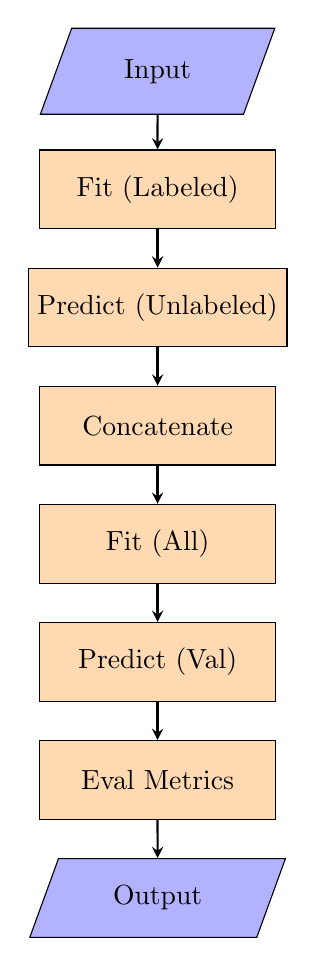
\begin{tikzpicture}[node distance=1.5 cm]
        % Nodes
        \node (input) [io] {Input};
        \node (fit_labeled) [process, below of=input] {Fit (Labeled)};
        \node (predict_unlabeled) [process, below of=fit_labeled] {Predict (Unlabeled)};
        \node (concatenate) [process, below of=predict_unlabeled] {Concatenate};
        \node (fit_all) [process, below of=concatenate] {Fit (All)};
        \node (predict_val) [process, below of=fit_all] {Predict (Val)};
        \node (eval_metrics) [process, below of=predict_val] {Eval Metrics};
        \node (output) [io, below of=eval_metrics] {Output};
        
        % Lines
        \draw [arrow] (input) -- (fit_labeled);
        \draw [arrow] (fit_labeled) -- (predict_unlabeled);
        \draw [arrow] (predict_unlabeled) -- (concatenate);
        \draw [arrow] (concatenate) -- (fit_all);
        \draw [arrow] (fit_all) -- (predict_val);
        \draw [arrow] (predict_val) -- (eval_metrics);
        \draw [arrow] (eval_metrics) -- (output);
    \end{tikzpicture}
    \caption{caption position}
\end{figure}



\begin{figure*}
    \centering
    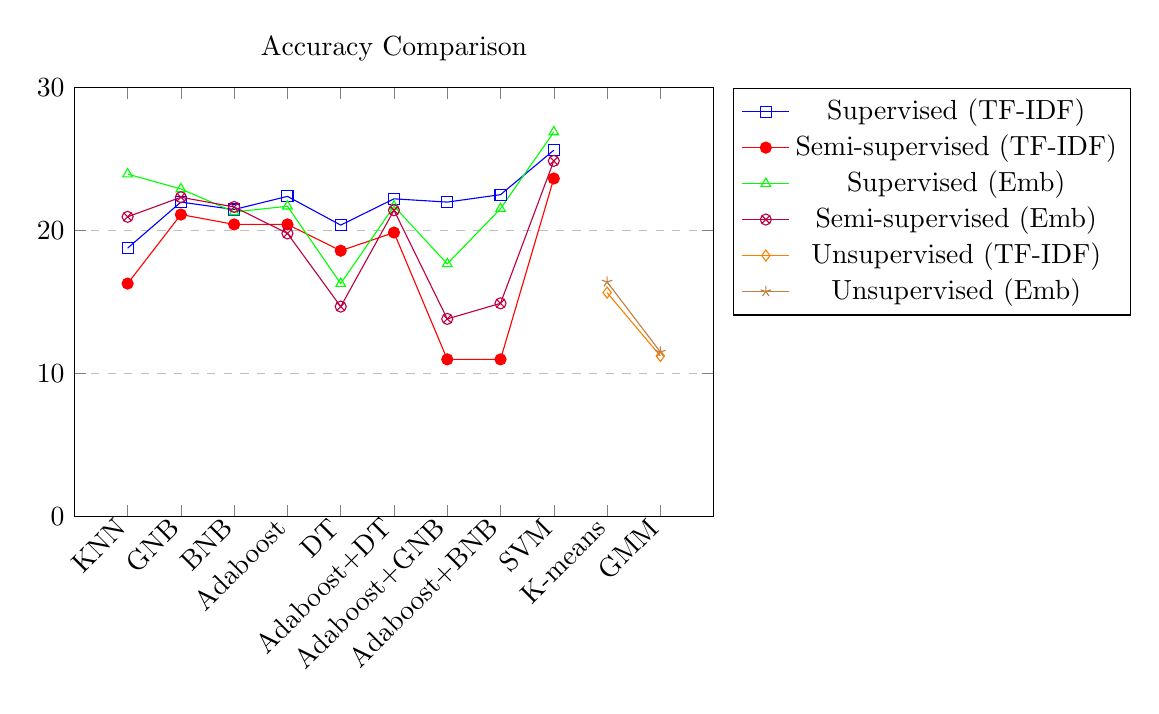
\begin{tikzpicture}
        \begin{axis}[
            title={Accuracy Comparison},
            % xlabel={Models},
            % ylabel={Accuracy},
            xmin=0, xmax=12,
            ymin=0, ymax=30,
            xtick={1, 2, 3, 4, 5, 6, 7, 8, 9, 10, 11, 12},
            xticklabels={
                KNN, GNB, BNB, Adaboost, DT, Adaboost+DT, Adaboost+GNB, Adaboost+BNB, SVM, K-means, GMM},
            xticklabel style={rotate=45, anchor=east},
            legend pos=outer north east,
            ymajorgrids=true,
            grid style=dashed,
            width=0.8\textwidth,
            height=200,
        ]
    
        % Labeled data (TFIDF)
        \addplot[
            color=blue,
            mark=square,
        ]
        coordinates {
            (1,18.77) (2,21.99) (3,21.47) (4,22.39) (5,20.38) (6,22.22) (7,21.99) (8,22.51) (9,25.62)
        };
        \addlegendentry{Supervised (TF-IDF)}
        
        % Unlabeled data (TFIDF)
        \addplot[
            color=red,
            mark=*,
        ]
        coordinates {
            (1,16.29) (2,21.12) (3,20.43) (4,20.43) (5,18.59) (6,19.86) (7,10.99) (8,10.99) (9,23.64)
        };
        \addlegendentry{Semi-supervised (TF-IDF)}
        
        % Labeled data (Embedding)
        \addplot[
            color=green,
            mark=triangle,
        ]
        coordinates {
            (1,23.95) (2,22.91) (3,21.3) (4,21.7) (5,16.29) (6,21.7) (7,17.67) (8,21.53) (9,26.89)
        };
        \addlegendentry{Supervised (Emb)}
    
        % Unlabeled data (Embedding) - Semi-supervised
        \addplot[
            color=purple,
            mark=otimes,
        ]
        coordinates {
            (1,20.96) (2,22.33) (3,21.65) (4,19.8) (5,14.68) (6,21.42) (7,13.82) (8,14.91) (9,24.87)
        };
        \addlegendentry{Semi-supervised (Emb)}
        
        % Unlabeled data (Embedding)
        \addplot[
            color=orange,
            mark=diamond,
        ]
        coordinates {
            (10,15.66) (11,11.23)
        };
        \addlegendentry{Unsupervised (TF-IDF)}

        \addplot[
            color=brown,
            mark=star,
        ]
        coordinates {
            (10,16.41) (11,11.51)
        };
        \addlegendentry{Unsupervised (Emb)}
        
        \end{axis}
    \end{tikzpicture}
\end{figure*}




\begin{table*}
    \begin{center}
        \captionof{table}{Accuracy Comparison} \label{tab:title} 
        \begin{tabularx}{\textwidth}{@{}l *{7}{>{\centering\arraybackslash}X} @{}}
        \toprule
        Model & \multicolumn{2}{c}{TFIDF} & \multicolumn{2}{c}{Embedding}\\
        \cmidrule(lr){2-3} \cmidrule(lr){4-5}
        & Labaled data & Unlabeled data & Labaled data & Unlabaled data \\
        \midrule
        
        	KNN & 18.77 & 16.29 & 23.95 & 20.96 \\
        	GNB & 21.99 & 21.12 & 22.91 & 22.33 \\
        	BNB  & 21.47 & 20.43 & 21.3 & 21.65 \\
        	Adaboost & 22.39 & 20.43 & 21.7 & 19.8 \\
        	Decision Tree (DT) & 20.38 & 18.59 & 16.29 & 14.68 \\
        	Adaboost + DT & 22.22 & 19.86 & 21.7 & 21.42 \\
        	Adaboost + GNB & 21.99 & 10.99 & 17.67 & 13.82 \\
        	Adaboost + BNB & 22.51 & 10.99 & 21.53 & 14.91 \\
        	SVM & \textbf{25.62}$^*$ & \textbf{24.64}$^*$ & \textbf{26.89}$^*$ & \textbf{24.87}$^*$ \\
        	\cmidrule(lr){1-5} 
        	K-means & - & \textbf{15.66}$^*$ & - & \textbf{16.41}$^*$ \\
        	GMM & - & 11.23 & - & 11.51 \\
        
        \bottomrule
        \end{tabularx}
        % \bigskip \vspace{In the dataset with labels, we use supervised machine learning algorithms. Then for the unlabelled part, we use self-training class supervised learning methods.}
        % \bigskip Should be a caption
    \end{center}
\end{table*}

\nocite{*}
\bibliographystyle{apalike}
\bibliography{sample}

\end{document}
